% OBS DETTA ÄR INTE EN OFFICIELL RAPPORTMALL
% OBS DETTA ÄR INTE EN OFFICIELL RAPPORTMALL
% OBS DETTA ÄR INTE EN OFFICIELL RAPPORTMALL

% OBS DETTA ÄR INTE EN OFFICIELL RAPPORTMALL
% OBS DETTA ÄR INTE EN OFFICIELL RAPPORTMALL
% OBS DETTA ÄR INTE EN OFFICIELL RAPPORTMALL
\documentclass[12pt,a4paper]{article}

\usepackage[utf8]{inputenc}


\usepackage[T1]{fontenc}
% För riktiga å, ä och ö:

% Den andra säger att vi ska använda fonter som är speciellt anpassade
% för Västeuropeiska språk, bland annat kommer prickarna över "ö" lite
% närmare o:et.
% Det räcker ofta, men inte alltid, att bara ange den senare. Det bör
% räcka att bara ange den första, men blir inte _fullt_ så snyggt.

\usepackage[swedish]{babel}
% Svensk avstavning (om den är installerad) och svenska rubriker på
% sådant som LaTeX lägger till: sammanfattning,
% innehållsförteckning...

\usepackage{mathtools}
% Paketet som tillåter en att skriva matematiska formler.

\usepackage{ae}
% När du gör PDF-filer för publicering på Internet eller för att
% skicka via e-post, bör du använda Type1-fonter (typsnitt). LaTeX
% använder vanligen bitmapfonter, som ger utmärkt resultat i skrivare,
% men bedrövligt på skärm. Med ae får du fonter med samma utseende som
% ordinarie LaTeX, men som också fungerar på bildskärmar. PDF-filer
% skapar du sedan genom att skriva "dvipdf filnamn" efter att ha kört
% LaTeX för att få fram en "filnamn.dvi".
%    Det finns ingen garanti för att alla fonter du använder finns med
% i ae, och de som inte finns kommer i regel få vanliga bitmapfonter
% istället. Men det rör sig då om enstaka stycken - kanske
% sammanfattningen du gjort med "abstract" till exempel - eller någon
% enstaka variabel. Det mesta blir bra.


\usepackage{listings}
% tillåter att formatera kod

\lstset{literate=%
{Ö}{{\"O}}1
{Ø}{{\O}}1
{Ä}{{\"A}}1
{Å}{{\AA}}1
{Ü}{{\"U}}1
{ß}{{\ss}}2
{ü}{{\"u}}1
{ä}{{\"a}}1
{å}{{\aa}}1
{ö}{{\"o}}1
{ø}{{\o}}1
{æ}{{\ae}}1
{Æ}{{\AE}}1
}
% Fixar så att åäö och andra tecken går att använda i kodfiler 

\renewcommand\appendix{\par
  \setcounter{section}{0}
  \setcounter{subsection}{0}
  \setcounter{figure}{0}
  \setcounter{table}{0}
  \renewcommand\thesection{Bilaga \Alph{section}}
  \renewcommand\thefigure{\Alph{section}\arabic{figure}}
}
%Lägger till rubriker för Bilagorna

\usepackage{units}
% Enheter ska skrivas i upprätt stil med seriffer, och separeras från
% föregående siffror med ett tunt mellanslag - tunnare än ett
% vanligt. Använd i texten/matteläget som: \unit[1,34]{m}

\usepackage{icomma}
% I icke-engelsk skrift används decimalkomma, i engelsk är kommatecken
% i matteläge enbart en koordinatavskiljare. Därför sätter LaTeX i
% vanliga fall automatiskt in ett extra mellanslag efter alla
% kommatecken i matteläge. Detta kommando ger ett intelligent
% kommatecken som förstår om det är decimalavskiljare eller
% koordinatavskiljare, beroende på om det står något mellanslag
% efter. Använd aldrig decimalpunkt i icke-engelsk skrift.

\usepackage{color}
\usepackage{graphics}
\usepackage{graphicx}
\usepackage{wrapfig}

% Dessa behövs när man inkluderar figurer från xfig, i
% latex+postscript format (brukar bli snyggast). Använder man vanliga
% eps-figurer behöver man inte color-paketet. Det finns både paketet
% "graphics" och "graphicx", med något olika syntax. Om alla bilder
% har rätt storlek när man importerar dem behöver man inte bry sig om
% skillnaderna. wrapfig tillåter en att skriva text runt en figur.

\usepackage{hyperref}

\usepackage{bbm}
\newcommand{\N}{\ensuremath{\mathbbm{N}}}
\newcommand{\Z}{\ensuremath{\mathbbm{Z}}}
\newcommand{\Q}{\ensuremath{\mathbbm{Q}}}
\newcommand{\R}{\ensuremath{\mathbbm{R}}}
\newcommand{\C}{\ensuremath{\mathbbm{C}}}
% Här hittar jag på nya kommandon för att beteckna mängden av de
% naturliga talen, heltalen, de rationella, de reella och de
% komplexa. Vill man ha en annan font kan man i stället använda
% \mathbb{N} och så vidare, men måste då inkludera följande rad:

\usepackage{amssymb}

\newcommand{\rd}{\ensuremath{\mathrm{d}}}
\newcommand{\id}{\ensuremath{\,\rd}}
% \rd står för rakt d, \id står för integral-d. Anledningen är att man
% ska kunna skilja på d som en variabel (diameter, avstånd) och d som
% en operator. I derivator och integraler ska d:et stå upprätt, och i
% integraler också med ett litet mellanrum mellan d och föregående
% uttryck.

\setlength\parindent{0pt}
%Tar bort intendering vid ny paragraf

\usepackage[backend=bibtex,
style=numeric
%style=alphabetic
%style=reading
]{biblatex}
\addbibresource{referenser}
% Möjlighet att skapa refernslista, med hjälp av BibTex-formatet.

\usepackage{rotating}
\usepackage[yyyymmdd]{datetime}
\renewcommand{\dateseparator}{-}
\usepackage[absolute]{textpos}



\begin{document}
%Innehåller vissa inställningar och hänvisningar till paket för att generera dokumentet

% OBS DETTA ÄR INTE EN OFFICIELL RAPPORTMALL
% OBS DETTA ÄR INTE EN OFFICIELL RAPPORTMALL
% OBS DETTA ÄR INTE EN OFFICIELL RAPPORTMALL
\begin{center}

% Skolans loggo, ShareLaTeX fixar inte eps-filer men pdf går bra därför har jag konventerat logotypen till pdf
% som också är vectorformat.

\includegraphics[width=12.2 cm]{Bilder/JTH_cmyk_B-eps-converted-to.pdf}\centering


 \begin{center}
\textsc{\LARGE  Rapport gruppuppgift 1\\diskussion och svar}\\[1.5cm]
% Rapportens rubrik, "\\" Anger ny rad. rymms namnet på en rad låt det vara på en rad. 


\textsc{\Large Kursnamnet}\\[0.5cm]
% Kursnamnet som rapporten ingår i.
\end{center}




\begin{textblock}{0.2}[0.5,0.2](0.9,13.4)
\begin{rotate}{90}
\footnotesize Kursstart ht -03 eller senare
\end{rotate}
\end{textblock}
 % Taget från JTHs ordinarie rapportmall, vet ej varför det finns där.
 
 
\vfill
\begin{flushleft} \large
\textsc{Kontaktperson:}
Eventuell \textsc{Kontaktperson}
% Kontaktperson om sådan finns

\textsc{Författare:}
Anders \textsc{Andersson} (DIS 2)
% Författarnamn, oftast dit namn.

\large
\textsc{Handledare:} 
Lärare \textsc{Larson}, Lärare \textsc{Olsson}
%Handledare oftast laborationsassistenten 

\textsc{Datum:}
\today 
% Datum för när rapporten kompilerades. 

\end{flushleft}

\end{center}
\thispagestyle{empty}
\pagebreak

\begin{abstract}
En kortare beskrivning på rapporten.
\end{abstract}
\setcounter{page}{1}
\newpage
\tableofcontents

\newpage
% Innehåller framsidan och innehållsförteckning


\section{Inleding}

En inledning för rapporten. Har du fler funderingar om LaTeX kan du läsa detta dokument: \href{http://upload.wikimedia.org/wikipedia/commons/2/2d/LaTeX.pdf}{\nolinkurl{LaTeX}}.

\section{Genomförande}
Förklarande text för hur arbetet gick till för att nå fram till resultat. \\ en ny rad. Formler går aldeles.
utmärt att köra i LaTeX.\\ 


\begin{math}
x_{1,2}=-\displaystyle\frac{p}{2}\pm\sqrt{\left(\displaystyle\frac{p}{2}\right)^2-q}
\end{math}
% Syntaxen som man skriver med kan vara lite svår att förstå till en början
% det finns en massa verktyg på internet som kan hjälpa dig
% http://www.sciweavers.org/free-online-latex-equation-editor


 \\  \\
KTH\footnote{Kungliga Tekniska Högskolan, är ett statligt svenskt universitet i Stockholm med huvudsaklig inriktning på teknik och naturvetenskap.} och Stockholms Universitet har en bra sida där man kan läsa hur man skriver formler \href{http://wiki.math.se/wikis/forberedandematte1/index.php/5.1_Skriva_matematiska_formler_i_LaTeX}{\nolinkurl{Här}}.
\\ \\
\newpage
\section{Resultat}
\subsection{\texttt{En valfri rubrik}}
En text till vad du fick fram för resultat, refererar till en bok \cite{einstein}.
Om man har haft en källa så är det väldigt viktigt att referera till källan \cite{einstein,latexcompanion}. Vi kan också inkludera bilder under texten.  Skulle bilden vara så omfattande så kan man hänvisa till en bilaga. Se \ref{tree:bilaga} för mer information.

\begin{figure}[ht]
    \centering
    \vspace{2mm}
    \scalebox{0.2}{
\includegraphics{Figurer/forever-alone-guy.png}}
	\caption{Helt ensam figur.}
	\label{fig:label}
\end{figure}

\subsection{\texttt{En till valfri rubrik}}
Tror du förstår nu, se \ref{hello:bilaga}.
Att notera när du infogar kod kan du inte använda åäö 


\lstset{tabsize=2,breaklines=true,numbers=left,basicstyle=\footnotesize,xleftmargin=30pt}
\lstinputlisting[language=C,]{Kod/helloWorld.c}
% Källkod i programspråket C inkluderas från filen helloWorld.c som ligger i mappen Kod. Läs  vilka språk som stöds http://en.wikibooks.org/wiki/LaTeX/Source_Code_Listings

\section{Diskussion}
Diskusion om vad som kan ha gjorts bättre och annat bra som kan vara bra att tillägga till varför resultatet blev som det blev. \\ \\ 
\begin{wrapfigure}{L}{45mm}
\vspace{-10pt}
  \begin{center}
    
\includegraphics[width=30mm]{Figurer/troll-face.png}
  \end{center}
  \vspace{-10pt}
  \caption{Ett troll}
  \vspace{-10pt}
\end{wrapfigure}

Detta är en text som syns vid sidan om en bild eller rättare sagt runt om en bild, när en bild syns brevid texten så kan bilden vara
ett verktyg till att få läsaren att förstå bättre. Det kan vara en graf eller helt enkelt en bild 
som beskriver ett flöde. Du kan bestämma avståndet mellan texten genom att ändra vspace. \\
Du kan ändra positionen på bilden också, om den skall vara till höger eller vänster sida, bara att ändra bokstaven brevid {wrapfigure} till  R eller L. Storleken på bilden ändras med width. Brevid {wrapfigure}{L} har du också ett mått, som bestämmer hur stort området skall vara som texten skall undvika.
\\ \\
Lorem ipsum dolor sit amet, consectetur adipiscing elit. Cras non ligula leo. Fusce eget cursus enim. Donec erat velit, suscipit eget hendrerit at, aliquam eu orci. Sed a faucibus enim. Fusce posuere tincidunt urna a mollis. Sed sed velit ac nibh dictum rutrum. Nunc congue pulvinar sem vitae sollicitudin. Morbi varius vulputate augue, et scelerisque erat dictum quis

\newpage
\addcontentsline{toc}{section}{Referenser}
\printbibliography


\appendix
\section{} \label{tree:bilaga}
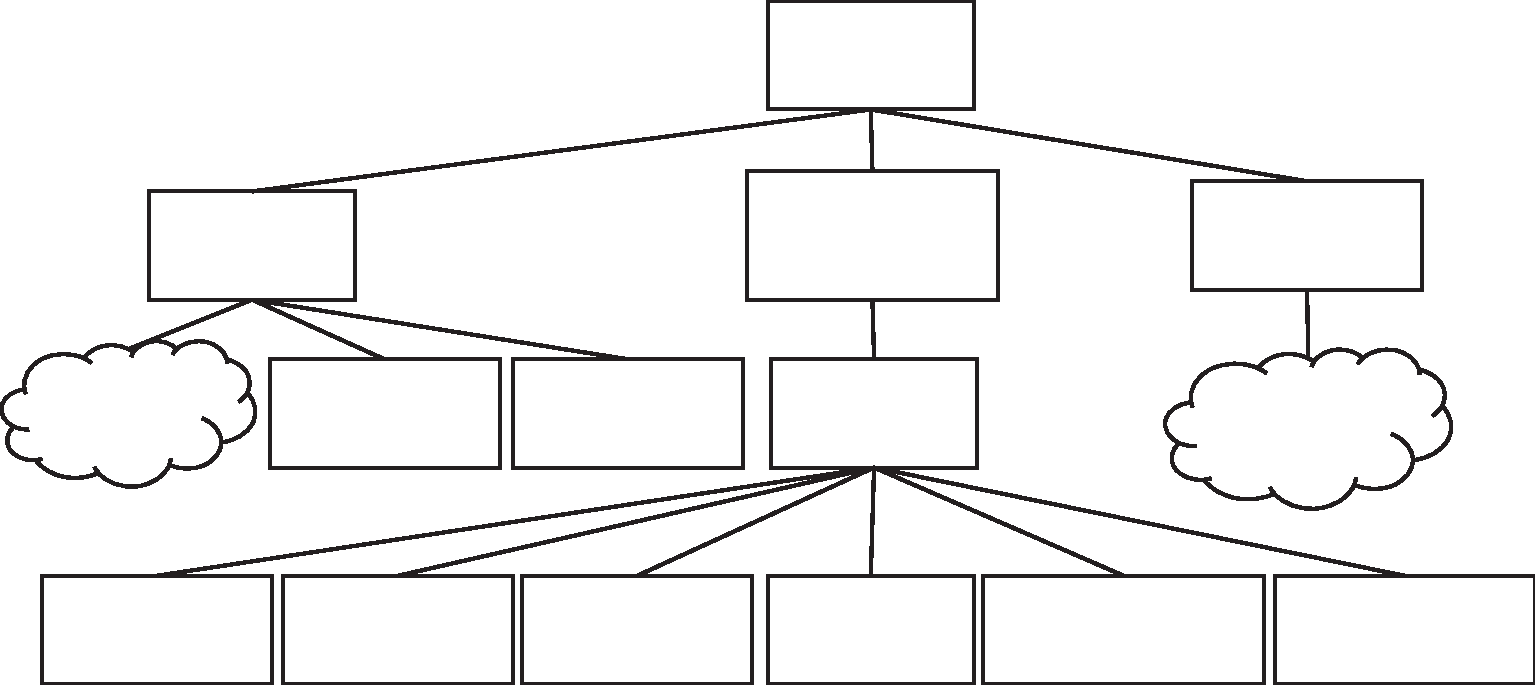
\includegraphics[angle=90,width=8.5 cm]{Bilagor/bilaga-eps-converted-to.pdf}\centering

\section{} \label{hello:bilaga}
\lstset{tabsize=2,breaklines=true,numbers=left,basicstyle=\footnotesize,xleftmargin=30pt}
\lstinputlisting[language=C,]{Kod/helloWorld.c}
% Källkod kan också vara bilaga Källkod, programspråket C inkluderas från filen helloWorld.c som ligger i mappen Kod. Läs  vilka språk som stöds http://en.wikibooks.org/wiki/LaTeX/Source_Code_Listings

\end{document}
